\documentclass[11pt,xcolor={rgb}]{beamer}

\usetheme{lagrange}

\usepackage{arev}
\usepackage{multicol}
\usepackage{listings}
\usepackage{amsmath,amssymb}
\usepackage[spanish]{babel}

\lstset{
  basicstyle=\ttfamily\color{accent2},
  frame=single,
}

\begin{document}

\title{Ajuste de Curvas: Interpolación de Lagrange}
\author{Bruno M. Breggia}
\institute{UNER - Facultad de Ingeniería}
\occasion{Programación Avanzada}
\date{10 de Mayo 2021}

\begin{frame}[plain]
\titlepage
\end{frame}

\section{Interpolaci\'on}

\begin{frame}
\frametitle{Interpolaci\'on}
\begin{center}
	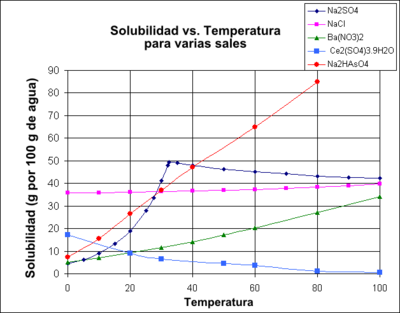
\includegraphics[scale=.6]{solubilidad}
	
\includegraphics[scale=.05]{solucion}
	\vfill
	Interpolaci\'on en qu\'imica
\end{center}
\end{frame}

\section{Interpolaci\'on de Lagrange}

\begin{frame}[fragile=singleslide]
\frametitle{Interpolamos con... polinomios}
Lagrange propone "unir los puntos" con un polinomio, dando mayor sensaci\'on de continuidad en toda la curva (derivadas continuas).
\begin{center}
	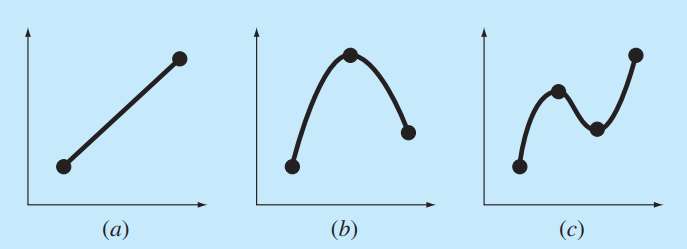
\includegraphics[scale=0.5]{interpolaciones}
	\vfill
	2 puntos $\rightarrow$ recta
	
	3 puntos $\rightarrow$ par\'abola
	
	4 puntos $\rightarrow$ c\'ubica
	
	...
\end{center}
\end{frame}

\begin{frame}[fragile=singleslide]
\frametitle{Fundamento matem\'atico}

Para un conjunto de $n$ puntos en el plano (de abscisas distintas), existe un y s\'olo un polinomio de grado $n-1$ que pase por todos esos puntos.
\linebreak

\textbf{Forma polin\'omica}
\begin{eqnarray}
f(x) &=& a_0 + a_1 x + a_2 x^2 + a_3 x^3 + ... + a_{n-1} x^{n-1}\\
f(x) &=& \sum\limits_{i=0}^{n-1}a_i x^i
\end{eqnarray}

Lagrange nos propone construir un polinomio de grado $n-1$ no a partir de sus coeficientes $\{a_0, a_1, ..., a_{n-1} \}$, sino a partir de $n$ puntos que pasan por \'el.

?`C\'omo lo hace?

\end{frame}


\begin{frame}[fragile=singleslide]
\frametitle{Armamos el interpolador de Lagrange}

Sup\'ongase que tenemos 3 puntos:

\begin{center}
\begin{multicols}{2}

	\begin{tabular}{c|c}
	X & Y\\	
	\hline
	$x_0$ & $y_0$\\
	$x_1$ & $y_1$\\
	$x_2$ & $y_2$
	\end{tabular}
	
	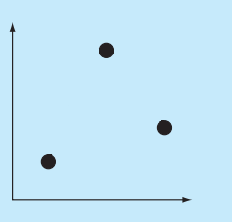
\includegraphics[scale=0.35]{puntos}

\end{multicols}
\end{center}

Queremos una funci\'on continua $f(x)$ que tome los valores $y_i$ correspondientes a cada valor $x_i$. Necesitamos algo de la forma:
$$f(x) = {\color{blue}L_0(x)}\ y_0 + {\color{blue}L_1(x)}\ y_1 + {\color{blue}L_2(x)}\ y_2$$
\linebreak
Los \textit{coeficientes variables} $L_i(x)$ son funciones que valen 1 s\'olo si $x = x_i$. Valen 0 si $x$ es igual a cualquier otro valor de abscisa de la tabla.

\end{frame}


\begin{frame}[fragile=singleslide]
\frametitle{Armamos el interpolador de Lagrange}

%Nuestra funci\'on es:
%$$f(x) = {\color{blue}L_0(x)}\ y_0 + {\color{blue}L_1(x)}\ y_1 + {\color{blue}L_2(x)}\ y_2$$

Los coeficientes $L_i(x)$ son \textit{polinomios}, y se denominan \textbf{Polinomios interpoladores de Lagrange}. Tenemos un $L(x)$ por cada punto conocido. Para el punto $(x_0,y_0)$ del ejemplo anterior, tenemos:

\[   
L_0(x) = 
     \begin{cases}
       1, &\quad\text{si}\ x=x_0\\
       0, &\quad\text{si}\ x = x_1,x_2 \\
     \end{cases}
\]

Los coeficientes $L_1, L_2$ siguen el mismo patr\'on. Si evaluamos $f(x)$ en $x_0$, tendremos...\\
\begin{eqnarray*}
f(x_0) &=& {\color{blue}L_0(x_0)}\ y_0 + {\color{blue}L_1(x_0)}\ y_1 + {\color{blue}L_2(x_0)}\ y_2\\
f(x_0) &=& {\color{blue}1}\ y_0 + {\color{blue}0}\ y_1 + {\color{blue}0}\ y_2\\
%f(x_0) &=& y_0
\end{eqnarray*}

Comprobamos que el punto $(x_0, y_0)$ pertenece a la funci\'on. Lo mismo ocurri\'a para los dem\'as puntos.

\end{frame}


\begin{frame}[fragile=singleslide]
\frametitle{Armamos el interpolador de Lagrange}

?`C\'omo se implementa $L_0(x)$?

Consideramos todos los valores $x_i$ (excepto $x_0$) como ra\'ices de un polinomio en forma factorizada. 
$${\color{blue}(x-x_1)(x-x_2)}\quad \rightarrow \quad \text{vale 0 si } x=x_1,x_2$$

Si $x=x_0$, queremos que nos d\'e la unidad, sin embargo, esta expresi\'on no resultar\'a necesariamente en uno:
$$(x_0-x_1)(x_0-x_2)$$

Para que nos d\'e la unidad, deberemos normalizarlo (dividir el polinomio por el valor anterior, el cual es una \textit{constante}).

$$\frac{{\color{blue}(x-x_1)(x-x_2)}}{(x_0-x_1)(x_0-x_2)}$$

Este polinomio vale 1 para $x_0$, y vale 0 para $x_1, x_2$. !`Hemos construido el polinomio interpolador de Lagrange para el primer t\'ermino de nuestra funci\'on interpolante!

\end{frame}


\begin{frame}[fragile=singleslide]
\frametitle{Armamos el interpolador de Lagrange}

Para finalizar, nuestra funci\'on interpolante es de la forma:
$$f(x) = {\color{blue}L_0(x)}\ y_0 + {\color{blue}L_1(x)}\ y_1 + {\color{blue}L_2(x)}\ y_2$$

Donde:
$${\color{blue}L_0(x)}=\frac{(x-x_1)(x-x_2)}{(x_0-x_1)(x_0-x_2)} \quad {\color{blue}L_1(x)}=\frac{(x-x_0)(x-x_2)}{(x_1-x_0)(x_1-x_2)} $$
$${\color{blue}L_2(x)}=\frac{(x-x_0)(x-x_1)}{(x_2-x_0)(x_2-x_1)}$$

\begin{multicols} {2}
Como los polinomios de Lagrange $L_i(x)$ son todos de 2do orden, la funci\'on interpolante $f(x)$ tambi\'en lo ser\'a.

\begin{center}
	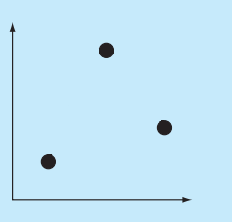
\includegraphics[scale=0.4]{puntos}
	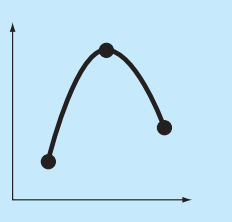
\includegraphics[scale=0.4]{puntos_interpolados}
\end{center}
\end{multicols}

\end{frame}


\begin{frame}[fragile=singleslide]
\frametitle{Armamos el interpolador de Lagrange}

\begin{center}
	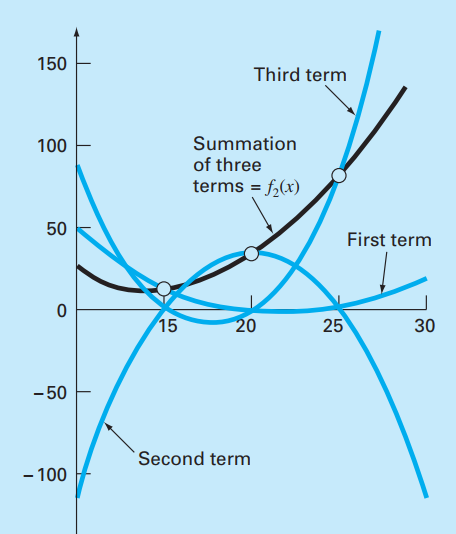
\includegraphics[scale=0.5]{lagrange_3puntos}
\end{center}

\end{frame}


\section{Formulaci\'on General}

\begin{frame}[fragile=singleslide]
\frametitle{La forma de Lagrange}

Un polinomio de grado $n-1$ puede expresarse como:
$$f(x) = \sum\limits_{i=0}^{n-1}y_i\ L_i(x)$$ 

Donde $L_i(x)$ es el \textit{polinomio interpolador de Lagrange}, y est\'a dado por:
$$L_i(x) = \prod_{\substack{j=0 \\ j\neq i}}^{n-1} \frac{x-x_j}{x_i-x_j}$$

De forma compacta, un polinomio en \textbf{forma de Lagrange} se expresa como:
$$f(x) = \sum\limits_{i=0}^{n-1}y_i\ \prod_{\substack{j=0 \\ j\neq i}}^{n-1} \frac{x-x_j}{x_i-x_j}$$ 

\end{frame}

%\begin{frame}[fragile=singleslide]
%\frametitle{Interpolamos con... polinomios}
%\begin{lstlisting}
%\documentclass[xcolor={rgb}]{beamer}
%
%\usetheme{lagrange}
%
%\begin{document}
%
%\begin{frame}
% Hello Beamer!
%\end{frame}
%
%\end{document}
%\end{lstlisting}
%Note that you \textcolor{accent3}{need to} use \lstinline!xcolor={rgb}! option for this theme.
%\end{frame}

\section{Algunas Desventajas}

\begin{frame}[fragile=singleslide]
\frametitle{Desventajas}

\textbf{Demasiado tiempo de c\'omputo} (complejidad $O(n^2)$): por cada punto a calcular se incurre en una doble iteraci\'on (una sumatoria y una productoria).

\textbf{Fen\'omeno de Runge}: oscilaciones en los extremos de intervalos discretos equiespaciados.

\begin{center}
	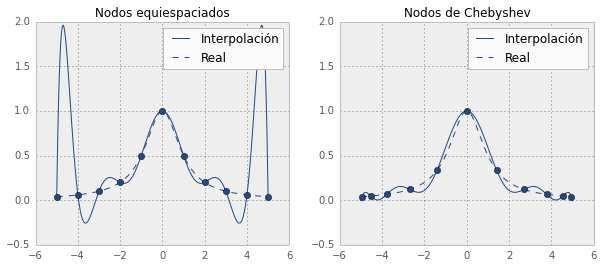
\includegraphics[scale=0.5]{runge1}
\end{center}


\end{frame}

%
%\begin{frame}[fragile=singleslide]
%\frametitle{Customization}
%To change vertical spaces between lines in TOC pages,
%you could redefine these two commands:
%\begin{lstlisting}
%\renewcommand{\sectionintochideskip}{10pt}
%\renewcommand{\sectionintocshowskip}{6pt}
%\end{lstlisting}
%\end{frame}

\end{document}